%----------------------------------------------------------------------------
%----------------------------------------------------------------------------
The envelope for the TEM00 mode from dye laser \#21 is calculated for the beam line described in figures \ref{dye_mileposts} and \ref{conditioning_table}. Equations \ref{free space} and \ref{thin lens} are used to propagate the complex source point $q$ down the beam line. We obtain the following complex source points for key points along the beam line ($\lambda=725$ nm):
%----------------------------------------------------------------------------
\begin{eqnarray}
q_{0}   &=& 1.346  + 8.495i,\\
q_{50}  &=& -1.022 + 0.114i,\\
q_{54}  &=& -3.144 + 5.885i,\\
q_{295} &=& -0.515 + 0.036i,
\end{eqnarray}
%----------------------------------------------------------------------------
where the subscript denotes the milepost at which the complex source is reported. See figure \ref{dye21_to_pinhole} for a plot of the beam envelope up to the pinhole.
%----------------------------------------------------------------------------
% dye21_to_pinhole.tex
% by Troy Hix, May 2005
%----------------------------------------------------------------------------
\begin{figure}
\centering
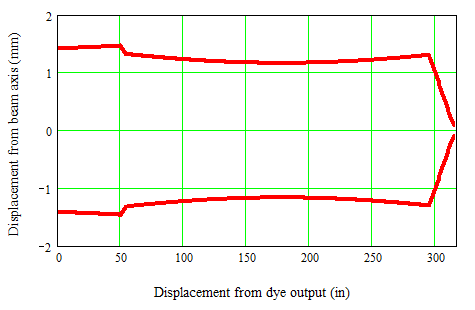
\includegraphics[width=4.00in]
{dye21_to_pinhole/dye21_to_pinhole.png}
\caption{TEM00 envelope for dye laser \#21}
\label{dye21_to_pinhole}
\end{figure} 
%----------------------------------------------------------------------------

%----------------------------------------------------------------------------
%----------------------------------------------------------------------------
%----------------------------------------------------------------------------
%----------------------------------------------------------------------------
%----------------------------------------------------------------------------
The beam lines for the three dye lasers are very similar. So, without corresponding plots like figure \ref{dye21_to_pinhole}, we report the complex source at key points along the beam lines for dye laser \#22 and \#23. For dye laser \#22 we have ($\lambda=628$ nm)
%----------------------------------------------------------------------------
\begin{eqnarray}
q_{0}   &=& 1.346  + 9.808i,\\
q_{50}  &=& -1.016 + 0.099i,\\
q_{55}  &=& -4.008 + 4.493i,\\
q_{344} &=& -0.515 + 0.040i;
\end{eqnarray}
%----------------------------------------------------------------------------
and for dye laser \#23 we have ($\lambda=872$ nm)
%----------------------------------------------------------------------------
\begin{eqnarray}
q_{0}   &=& 1.346  + 7.063i,\\
q_{50}  &=& -1.031 + 0.135i,\\
q_{52.5}&=& -0.707 + 7.018i,\\
q_{280} &=& -0.516 + 0.025i.
\end{eqnarray}
%----------------------------------------------------------------------------
Note that the initial complex source point is slightly different for each laser. This is because the waist was fixed and the Rayleigh parameter was recalculated given the different wavelength of each laser.
%----------------------------------------------------------------------------
%----------------------------------------------------------------------------
%----------------------------------------------------------------------------
%----------------------------------------------------------------------------
